% abtex2-modelo-artigo.tex, v-1.9.2 laurocesar
% Copyright 2012-2014 by abnTeX2 group at http://abntex2.googlecode.com/ 
%

% ------------------------------------------------------------------------
% ------------------------------------------------------------------------
% abnTeX2: Modelo de Artigo Acadêmico em conformidade com
% ABNT NBR 6022:2003: Informação e documentação - Artigo em publicação 
% periódica científica impressa - Apresentação
% ------------------------------------------------------------------------
% ------------------------------------------------------------------------

\documentclass[
	% -- opções da classe memoir --
	article,			% indica que é um artigo acadêmico
	11pt,				% tamanho da fonte
	oneside,			% para impressão apenas no verso. Oposto a twoside
	a4paper,			% tamanho do papel. 
	% -- opções da classe abntex2 --
	%chapter=TITLE,		% títulos de capítulos convertidos em letras maiúsculas
	%section=TITLE,		% títulos de seções convertidos em letras maiúsculas
	%subsection=TITLE,	% títulos de subseções convertidos em letras maiúsculas
	%subsubsection=TITLE % títulos de subsubseções convertidos em letras maiúsculas
	% -- opções do pacote babel --
	english,			% idioma adicional para hifenização
	brazil,				% o último idioma é o principal do documento
	sumario=tradicional
	]{abntex2}


% ---
% PACOTES
% ---

% ---
% Pacotes fundamentais 
% ---
\usepackage{lmodern}			% Usa a fonte Latin Modern
\usepackage[T1]{fontenc}		% Selecao de codigos de fonte.
\usepackage[utf8]{inputenc}		% Codificacao do documento (conversão automática dos acentos)
\usepackage{indentfirst}		% Indenta o primeiro parágrafo de cada seção.
\usepackage{nomencl} 			% Lista de simbolos
\usepackage{color}				% Controle das cores
\usepackage{graphicx}			% Inclusão de gráficos
\usepackage{microtype} 			% para melhorias de justificação
% ---
		
% ---
% Pacotes adicionais, usados apenas no âmbito do Modelo Canônico do abnteX2
% ---
\usepackage{lipsum}				% para geração de dummy text
% ---
		
% ---
% Pacotes de citações
% ---
\usepackage[brazilian,hyperpageref]{backref}	 % Paginas com as citações na bibl
\usepackage[alf]{abntex2cite}	% Citações padrão ABNT
% ---

% ---
% Pacotes extras
% ---
\usepackage{amsmath}    % Pacote para matemática
\usepackage{float}      % Pacote para controle de formatação de imagens 
                        % e tabelas

% ---
% Configurações do pacote backref
% Usado sem a opção hyperpageref de backref
\renewcommand{\backrefpagesname}{Citado na(s) página(s):~}
% Texto padrão antes do número das páginas
\renewcommand{\backref}{}
% Define os textos da citação
\renewcommand*{\backrefalt}[4]{
	\ifcase #1 %
		Nenhuma citação no texto.%
	\or
		Citado na página #2.%
	\else
		Citado #1 vezes nas páginas #2.%
	\fi}%
% ---

% ---
% Informações de dados para CAPA e FOLHA DE ROSTO
% ---
\titulo{Problema 1: Rega Automatizada!}
\autor{
    Cláudio Daniel Figueredo Peruna \thanks{danielperuna2012@gmail.com} 
    \and Paulo Gabriel da Rocha Costa Silva \thanks{paulogrcsilva@gmail.com}
    \and Paulo Henrique Dantas Barreto \thanks{rickdeuxvult@gmail.com}
}
\local{Feira de Santana - Bahia}
\data{2024}
% ---

% ---
% Configurações de aparência do PDF final

% alterando o aspecto da cor azul
\definecolor{blue}{RGB}{41,5,195}

% informações do PDF
\makeatletter
\hypersetup{
     	%pagebackref=true,
		pdftitle={\@title}, 
		pdfauthor={\@author},
    	pdfsubject={Modelo de artigo científico com abnTeX2},
	    pdfcreator={LaTeX with abnTeX2},
		pdfkeywords={abnt}{latex}{abntex}{abntex2}{atigo científico}, 
		colorlinks=true,       		% false: boxed links; true: colored links
    	linkcolor=blue,          	% color of internal links
    	citecolor=blue,        		% color of links to bibliography
    	filecolor=magenta,      		% color of file links
		urlcolor=blue,
		bookmarksdepth=4
}
\makeatother
% --- 

% ---
% compila o indice
% ---
\makeindex
% ---

% ---
% Altera as margens padrões
% ---
\setlrmarginsandblock{3cm}{3cm}{*}
\setulmarginsandblock{3cm}{3cm}{*}
\checkandfixthelayout
% ---

% --- 
% Espaçamentos entre linhas e parágrafos 
% --- 

% O tamanho do parágrafo é dado por:
\setlength{\parindent}{1.3cm}

% Controle do espaçamento entre um parágrafo e outro:
\setlength{\parskip}{0.2cm}  % tente também \onelineskip

% Espaçamento simples
\SingleSpacing

% ----
% Início do documento
% ----
\begin{document}

% Retira espaço extra obsoleto entre as frases.
\frenchspacing 

% ----------------------------------------------------------
% ELEMENTOS PRÉ-TEXTUAIS
% ----------------------------------------------------------

%---
%
% Se desejar escrever o artigo em duas colunas, descomente a linha abaixo
% e a linha com o texto ``FIM DE ARTIGO EM DUAS COLUNAS''.
% \twocolumn[    		% INICIO DE ARTIGO EM DUAS COLUNAS
%
%---
% página de titulo
\maketitle

% resumo em português
\begin{resumoumacoluna}
 Este relatório visa apresentar a metodologia e o desenvolvimento de um sistema automatizado de irrigação. O sistema foi projetado para otimizar o uso da água em plantações, buscando aprimorar a eficiência econômica em comparação aos métodos tradicionais de irrigação. Utilizando a linguagem de programação \textit{Verilog estrutural} e o \textit{software} \textit{Quartus}, o sistema foi implementado em uma placa \textit{CPLD MAX II}. Os resultados alcançados confirmaram o sucesso do projeto, demonstrando a viabilidade técnica e a eficácia operacional do sistema proposto. Além disso, o projeto contribuiu para a consolidação de conhecimentos teóricos relacionados a Sistemas Digitais, corroborando com a literatura existente e indicando caminhos para futuras pesquisas e aplicações práticas no campo da automação agrícola.
 
 \vspace{\onelineskip}
 
 \noindent
 \textbf{Palavras-chaves}: irrigação automatizada. circuitos digitais. verilog. quartus. CPLD MAX II. eficiência hídrica. sistemas digitais. tecnologia agrícola.
\end{resumoumacoluna}

% ]  				% FIM DE ARTIGO EM DUAS COLUNAS
% ---

% ----------------------------------------------------------
% ELEMENTOS TEXTUAIS
% ----------------------------------------------------------
\textual

% ----------------------------------------------------------
% Introdução
% ----------------------------------------------------------
\section*{Introdução}

A eficiência agrícola é um tema de suma importância para a sociedade e estudado há anos. Um exemplo é a Revolução Verde, que foi uma proposta iniciada na década de 30 buscando revolucionar o sistema agrícola internacional ao aprimorar sua produção, segundo \cite{zambenedetti_2021_revoluo}. 
Para atingir seus objetivos, essa proposta visava o uso de técnicas modernas como o uso de organismos geneticamente melhorados, uso de mecanização, como também o uso de irrigação automatizada.

Pensando nestes benefícios, este projeto tem como objetivo de desenvolver um protótipo de sistema automático de irrigação. Para tal, foi utilizado o \textit{Kit CPLD-LEDS}, que utiliza a placa \textit{CPLD MAX II} para então simular o ambiente e interface de interação com o usuário. 
Os interruptores foram usados para simular os sensores de níveis da caixa d’água e de ambiente, assim como a escolha da opção do menu pelo usuário, o barramento de LEDs para simular a abertura das válvulas, o LED RGB para o alarme, e o \textit{display} de sete segmentos, para o painel de informações.


% ----------------------------------------------------------
% Seção de Metodologia
% ----------------------------------------------------------

\section{Metodologia}

\subsection{Ferramentas Utilizadas}

O \textit{Kit de Desenvolvimento LEDS-CPLD} fora utilizada para a realização do projeto, a placa utilizada é a \textit{EPM240T100C5N} da família \textit{MAX II}; a linguagem de descrição de hardware utilizada fora o \textit{Verilog HDL}, e seu compilador, o \textit{Quartus II} da \textit{Intel} nas versões 18 e 20; 
Já como editor de código, fora utilizado o próprio \textit{Quartus II} e, em certos momentos, o \textit{Visual Studio Code} da \textit{Microsoft}. 
\textit{Python 3.10} foi utilizado como ferramenta auxiliar para gerar os arquivos de configuração e limpar o projeto após compilado, assim como o \textit{Git} fora usado para versionamento do código, e o \textit{Github} como repositório remoto.

\subsubsection{Visão Geral}

Para facilitar a compreensão da arquitetura do sistema proposto, recomenda-se a análise do fluxograma geral do circuito, apresentado na Figura \ref{fig:overview}.
\begin{figure}[H]
    \centering
    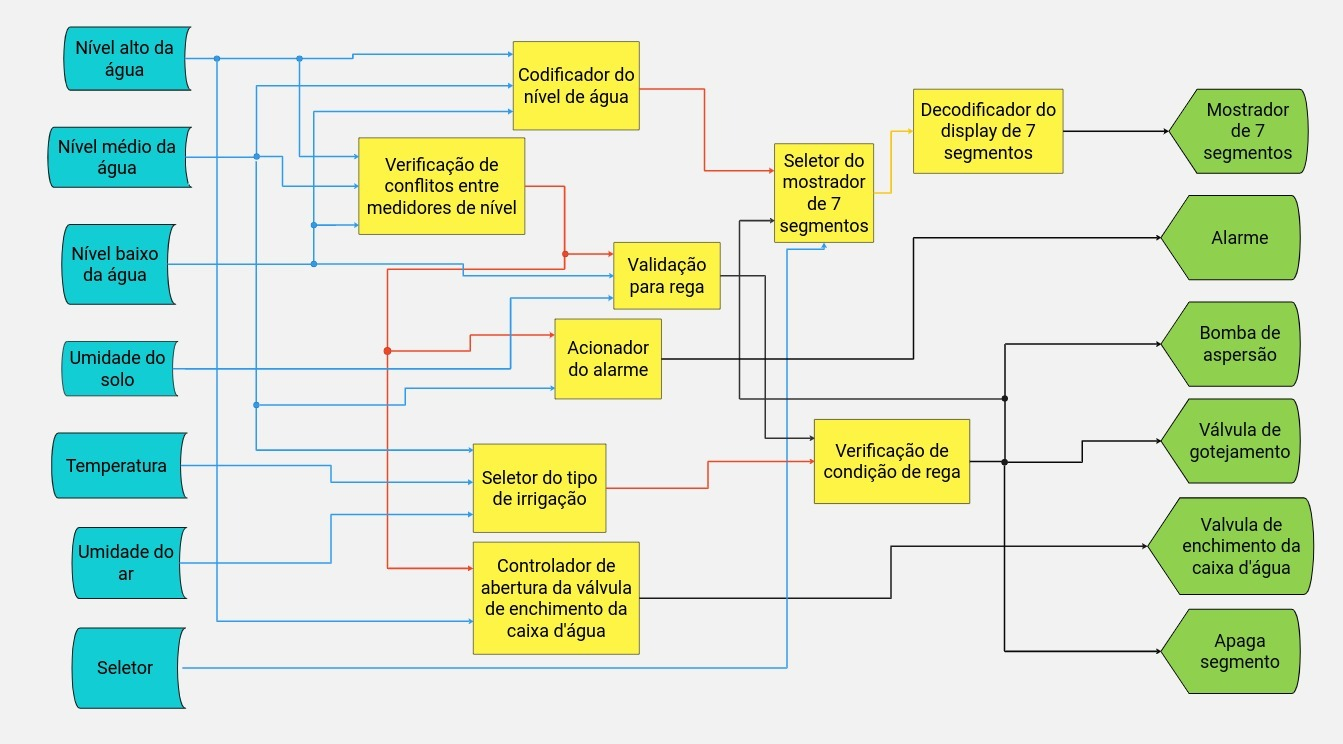
\includegraphics[width=0.75\linewidth]{full-view.png}
    \caption{Visão Geral do projeto}
    \label{fig:overview}
\end{figure}

Através deste, é possível identificar a estratégia de modularização adotada, que consiste na verificação sistemática dos níveis da caixa d’água (alto, médio e baixo). Esta verificação é realizada por meio de um algoritmo de detecção de conflitos entre os sensores, assegurando que as combinações de sinais sejam coerentes e livres de erros, antes de prosseguir para a etapa de codificação dos dados.

A saída do processo de verificação é direcionada para um controlador responsável pela operação da válvula de enchimento da caixa d’água, que também é influenciado pelo sensor de nível alto. Paralelamente, o seletor de irrigação processa entradas provenientes do sensor de nível médio da água, além dos sensores de temperatura e umidade do ar, para determinar as condições adequadas de irrigação.

O sistema de alarme é acionado com base no nível médio da água e nos resultados da verificação de conflitos, alertando sobre quaisquer discrepâncias ou condições críticas. Finalmente, o decodificador do display de 7 segmentos interpreta os sinais do seletor para exibir informações pertinentes ao tipo de irrigação empregado ou ao nível atual da caixa d’água.

\subsubsection{Imagens da Placa}

A interface do usuário do sistema é projetada para exibir uma variedade de informações através de um \textit{display} de 7 segmentos, um LED RGB e uma barra de LEDs. Esses componentes fornecem uma representação visual das condições operacionais do sistema, conforme descrito na Seção 1.3 (Pinagem).

Quando o \textit{display} de 7 segmentos é configurado para indicar o nível da água na caixa, quatro estados distintos podem ser representados: nível crítico (Figura \ref{fig:critic}), nível baixo (Figura \ref{fig:low}), nível médio (Figura \ref{fig:mid}) e nível alto (Figura \ref{fig:high}). Cada estado é associado a uma imagem específica no \textit{display}, permitindo uma identificação rápida e intuitiva do status atual da caixa d’água.

\begin{figure}[H]
    \centering
    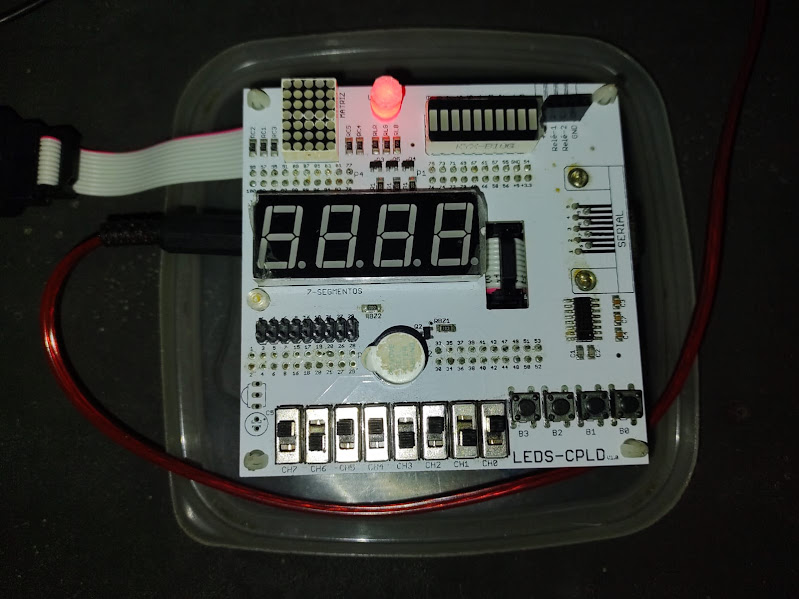
\includegraphics[width=0.5\linewidth]{display-critic.png}
    \caption{Nível crítico da caixa d'água}
    \label{fig:critic}
\end{figure}
\begin{figure}[H]
    \centering
    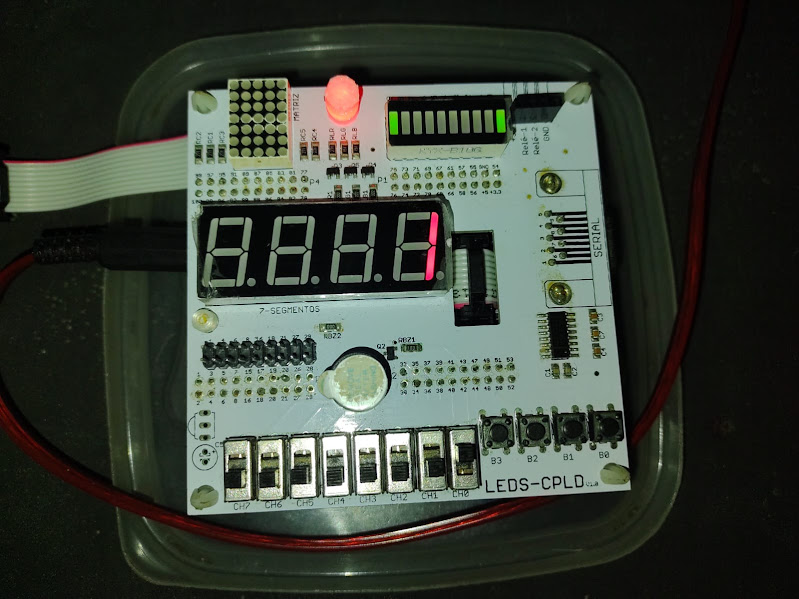
\includegraphics[width=0.5\linewidth]{low.png}
    \caption{Nível baixo da caixa d'água}
    \label{fig:low}
\end{figure}
\begin{figure}[H]
    \centering
    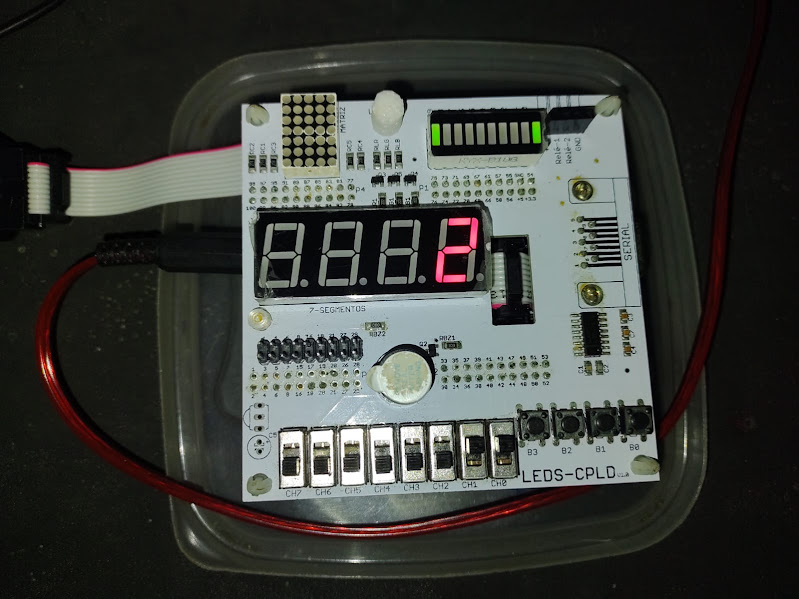
\includegraphics[width=0.5\linewidth]{mid.png}
    \caption{Nível médio da caixa d'água}
    \label{fig:mid}
\end{figure}
\begin{figure}[H]
    \centering
    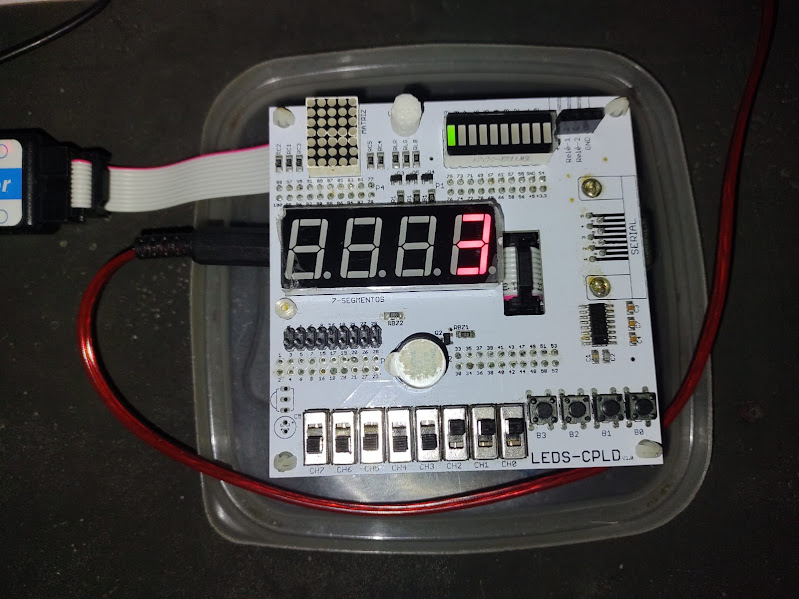
\includegraphics[width=0.5\linewidth]{high.png}
    \caption{Nível alto da caixa d'água}
    \label{fig:high}
\end{figure}

Além disso, o seletor do \textit{display} pode ser ajustado para mostrar o modo de irrigação em operação. Neste caso, três imagens são possíveis: a representação da irrigação por aspersão (Figura \ref{fig:asp}), a irrigação por gotejamento, e uma indicação do estado do alarme (ativo, na Figura \ref{fig:got-atv} ou inativo, na Figura \ref{fig:got-inatv}), que é determinado pela análise dos sinais dos sensores. É importante notar que os modos de irrigação são visualizados não apenas no \textit{display} de 7 segmentos, mas também na barra de LEDs, proporcionando uma dupla confirmação do tipo de irrigação selecionado.

\begin{figure}[H]
    \centering
    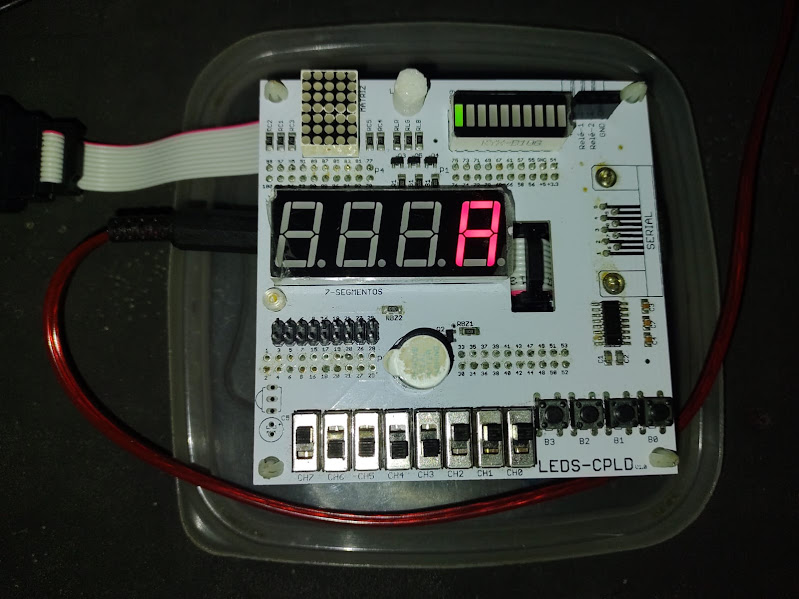
\includegraphics[width=0.5\linewidth]{aspersao.png}
    \caption{Bomba de Aspersão ativada}
    \label{fig:asp}
\end{figure}
\begin{figure}[H]
    \centering
    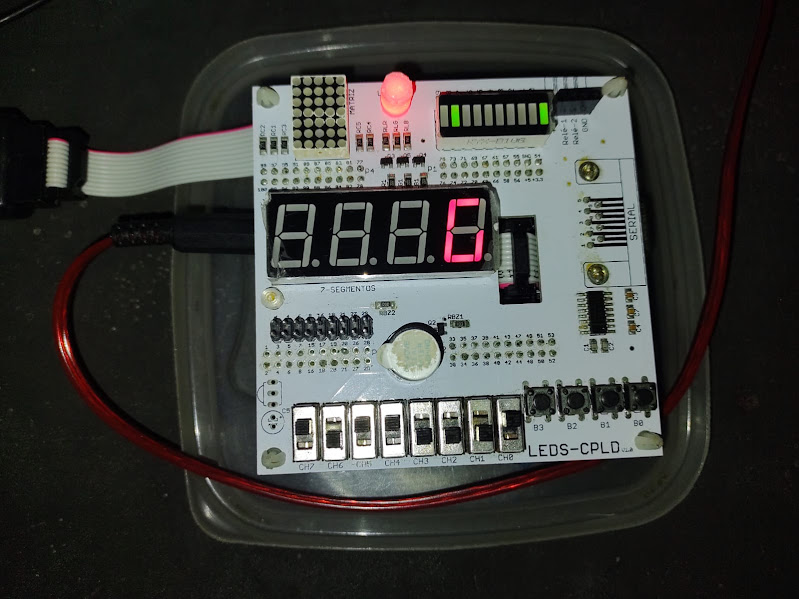
\includegraphics[width=0.5\linewidth]{got-atv.png}
    \caption{Válvula de Gotejamento ativada, com Alarme ligado}
    \label{fig:got-atv}
\end{figure}
\begin{figure}[H]
    \centering
    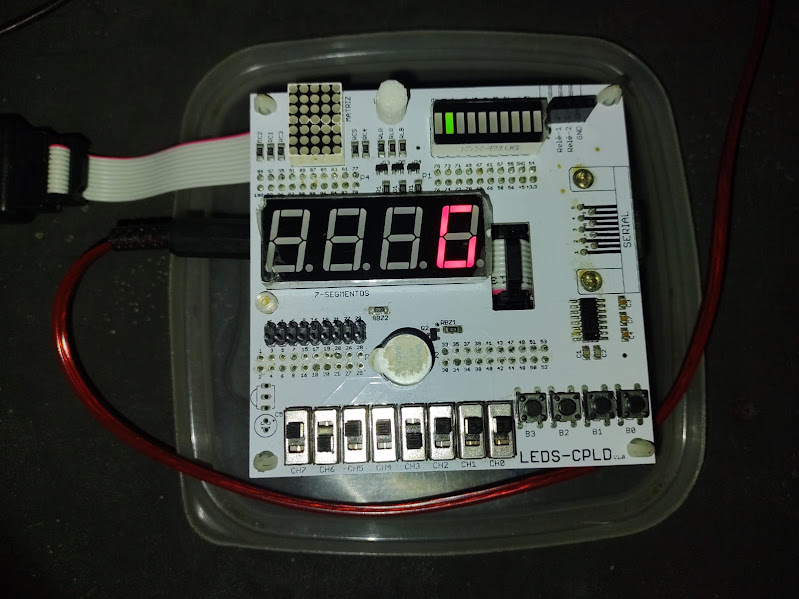
\includegraphics[width=0.5\linewidth]{got-inatv.png}
    \caption{Válvula de Gotejamento ativada, com Alarme desligado}
    \label{fig:got-inatv}
\end{figure}

\subsection{Escrita do código e Documentação}

Na implementação do código-fonte, adotou-se uma metodologia que prioriza a legibilidade e a manutenção do software. Utilizaram-se variáveis semânticas para garantir clareza e autoexplicabilidade, minimizando assim a necessidade de comentários adicionais. A redução de ruído foi alcançada por meio da eliminação de elementos supérfluos e da utilização de nomes para instâncias apenas quando estritamente necessário, seguindo as melhores práticas de codificação.

Em relação à documentação, cada módulo foi meticulosamente documentado, descrevendo suas funcionalidades e o papel que desempenham dentro da arquitetura do sistema. Esta documentação detalhada é fundamental para a compreensão do projeto como um todo, facilitando a integração de novos colaboradores e a expansão futura do sistema.

\subsection{Módulos}

Optou-se pela modularização do problema em questão, visando uma série de benefícios intrínsecos a essa abordagem. A divisão em módulos distintos permite não apenas uma manutenção mais eficiente, mas também facilita a visualização e otimização do projeto como um todo. Os módulos propostos são delineados a seguir, cada um com suas respectivas funções e interfaces claramente definidas, permitindo assim uma integração coesa e uma colaboração interdisciplinar efetiva. 

\subsubsection{Alarme}

O módulo de alarme, \textit{alarm.v}, é responsável por indicar baixo nível de água ou conflitos nos sensores da caixa d’água. 
Ele possui duas entradas: uma que indica se o nível de água está abaixo do nível médio, \textit{mid\_water\_level}, e outra que indica se há valores conflitantes dos sensores da caixa d'água, \textit{conflicting\_values}. 
A saída do módulo, representado por \textit{alarm\_on}, é um sinal que controla o estado do alarme. 

Sua representação em tabela verdade pode ser visto na Tabela \ref{tab:alarm}, assim como sua simplificação usando produto das somas pode ser visto na Equação \eqref{math:alarm} e seu esquema pode ser visto na Figura \ref{fig:alarm}.

\begin{table}[h]
\centering
\begin{tabular}{|c|c|c|c|}
\hline
\textit{mid\_water\_level} & \textit{conflicting\_values} & \textit{} & \textit{alarm\_on} \\ \hline
0 & 0 &  & 1 \\ \hline
0 & 1 &  & 1 \\ \hline
1 & 0 &  & 0 \\ \hline
1 & 1 &  & 1 \\ \hline
\end{tabular}
\caption{Tabela verdade do módulo \textit{alarm.v}}
\label{tab:alarm}
\end{table}

\begin{equation}
alarm\_on = mid\_water\_level' + conflicting\_values
\label{math:alarm}
\end{equation}

\begin{figure}[H]
    \centering
    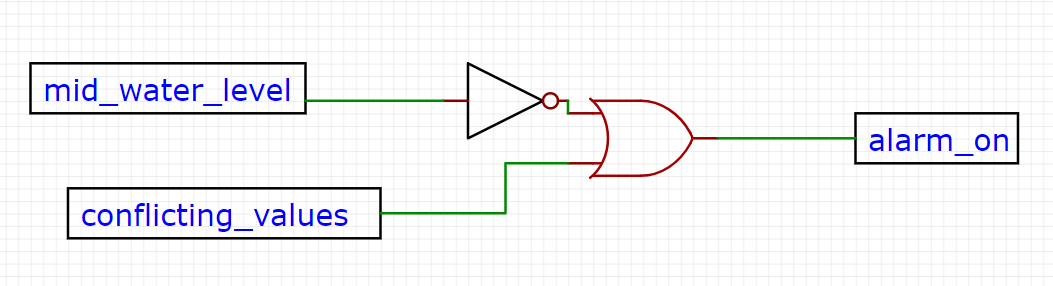
\includegraphics[width=0.75\linewidth]{alarm.png}
    \caption{Esquema do alarme}
    \label{fig:alarm}
\end{figure}

\subsubsection{Verificadores de conflitos nos sensores da caixa d’água}

O módulo \textit{water\_sensors\_checker.v} tem como finalidade verificar se existem valores conflitantes entre os sensores de nível de água do sistema. 
Esta verificação é crucial para garantir a precisão das leituras dos níveis de água e evitar operações inconsistentes do sistema de irrigação.

O módulo possui três entradas correspondentes aos diferentes sensores de nível de água: baixo (\textit{low\_level}), médio (\textit{mid\_level}) e alto (\textit{high\_level}). 
Sua saída é o sinal \textit{conflict}, que indica se há conflito entre os valores dos sensores.

Logo abaixo estão a tabela verdade em Tabela \ref{tab:sensor-checker} do módulo, assim como sua simplificação usando soma de produtos na Equação \eqref{math:checker}. Para fins didáticos, a equação utiliza outros nomes mais simples para se referir às entradas. Por tanto, \textit{A} é equivalente a \textit{high\_level}, \textit{B} a \textit{mid\_level}, \textit{C} a \textit{low\_level} e \textit{Z} a \textit{conflict}. Seu esquema pode ser visto na Figura \ref{fig:error}.


\begin{table}[h]
\centering
\begin{tabular}{|c|c|c|l|c|}
\hline
\textit{high\_level} & \multicolumn{1}{l|}{\textit{mid\_level}} & \textit{low\_level} &  & \textit{conflict} \\ \hline
0 & 0 & 0 &  & 0 \\ \hline
0 & 0 & 1 &  & 1 \\ \hline
0 & 1 & 0 &  & 1 \\ \hline
0 & 1 & 1 &  & 0 \\ \hline
1 & 0 & 0 &  & 1 \\ \hline
1 & 0 & 1 &  & 1 \\ \hline
1 & 1 & 0 &  & 1 \\ \hline
1 & 1 & 1 &  & 0 \\ \hline
\end{tabular}
\caption{Tabela verdade do módulo water\_sensors\_checker.v}
\label{tab:sensor-checker}
\end{table}

\begin{equation}
\begin{split}
Z &= A'BC' + AB'C' + AB'C + ABC' \\
Z &= A'BC' + A(B'C' + B'C)  + ABC'\\
Z &= A'BC' + AB' + ABC' \\
Z &= C'(A'B + AB) + AB' \\
Z &= C'B + AB' \equiv A'B + B'C
\label{math:checker}
\end{split}
\end{equation}

\begin{figure}[H]
    \centering
    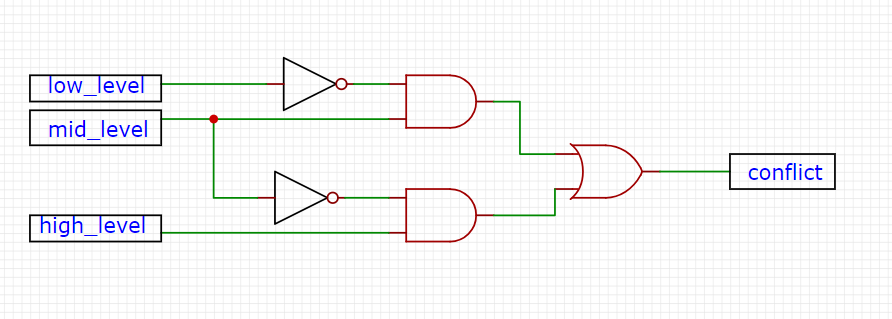
\includegraphics[width=0.75\linewidth]{error.png}
    \caption{Esquema da verificação de conflitos entre os sensores da caixa d'água}
    \label{fig:error}
\end{figure}



\subsubsection{Controlador do suprimento da caixa d’água}

O módulo \textit{water\_supply\_controller} é responsável por controlar a válvula de fornecimento de água em um sistema. 
Sua função é garantir que a válvula permaneça fechada em determinadas condições específicas, conforme as seguintes regras:

A válvula deve permanecer fechada se houver valores conflitantes provenientes dos sensores de nível de água. 
Isso é necessário para evitar operações inconsistentes do sistema de irrigação que podem resultar de leituras imprecisas dos sensores.

A válvula deve permanecer fechada quando o reservatório de água estiver cheio, ou seja, quando o nível de água estiver alto.
Isso é essencial para evitar o desperdício de água e possíveis danos causados por transbordamento.

Sua representação na tabela verdade pode ser vista em \textit{Tabela \ref{tab:water-supply}}, e sua simplificação por meio de soma de produtos pode ser encontrada na \textit{Equação} \eqref{math:supply}, no código em \textit{Verilog}, porém, a lógica é implementada por meio de uma porta \textit{NOR}, isso se deve à simplificação por meio do Teorema de DeMorgan como demonstrado por \cite{floyd_2007_lgebra}, e seu esquema na Figura \ref{fig:ve}.

\begin{table}[h]
\centering
\begin{tabular}{|c|c|c|c|}
\hline
\textit{water\_sensors\_conflicting,} & \multicolumn{1}{l|}{\textit{high\_water\_level}} & \textit{} & \textit{valvule} \\ \hline
0 & 0 &  & 1 \\ \hline
0 & 1 &  & 0 \\ \hline
1 & 0 &  & 0 \\ \hline
1 & 1 &  & 0 \\ \hline
\end{tabular}
\caption{Tabela verdade do módulo \textit{water\_supply\_controller.v}}
\label{tab:water-supply}
\end{table}


\begin{equation}
\begin{split}
valvule &= water\_sensors\_conflicting' \times high\_water\_level'  \\
& \text{Aplicando Teorema de DeMorgan} \\
valvule &= (water\_sensors\_conflicting + high\_water\_level)'
\label{math:supply}
\end{split}
\end{equation}

\begin{figure}[H]
    \centering
    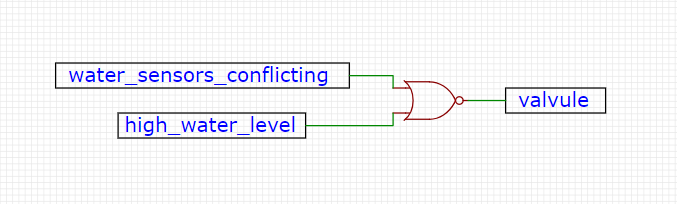
\includegraphics[width=0.75\linewidth]{Ve.png}
    \caption{Esquema da abertura entrada de água}
    \label{fig:ve}
\end{figure}

\subsubsection{Codificador do nível da caixa d’água}

O módulo \textit{Verilog} denominado \textit{water\_encoder} tem como função codificar o nível de água em um sistema, atribuindo bits a diferentes estados de nível de água. 
Essa codificação é essencial para o funcionamento do decodificador, possibilitando a representação adequada do nível de água em dispositivos de exibição, como demonstrado por \cite{floyd_2007_funes}.

O módulo possui três entradas correspondentes aos diferentes estados de nível de água: alto (\textit{high}), médio (\textit{mid}) e baixo (\textit{low}). As saídas do módulo consistem em dois bits codificados (\textit{encoded\_water\_Bit0} e \textit{encoded\_water\_Bit1}), que representam os diferentes níveis de água de acordo com a codificação especificada.

O representação da tabela verdade do módulo pode ser encontrada na Tabela \ref{tab:water-level-encoder}, e sua simplificação na Equação \eqref{math:water-level-encoder-0} e \eqref{math:water-level-encoder-1}, usando o método de soma de produtos.

\begin{table}[h]
\centering
\begin{tabular}{|c|c|c|c|c|c|}
\hline
high & mid & low &  & bit0 & bit1 \\ \hline
0    & 0   & 0   &  & 0    & 0    \\ \hline
0    & 0   & 1   &  & 0    & 1    \\ \hline
0    & 1   & 0   &  & 0    & 0    \\ \hline
0    & 1   & 1   &  & 1    & 0    \\ \hline
1    & 0   & 0   &  & 0    & 0    \\ \hline
1    & 0   & 1   &  & 0    & 0    \\ \hline
1    & 1   & 0   &  & 0    & 0    \\ \hline
1    & 1   & 1   &  & 1    & 1    \\ \hline
\end{tabular}
\caption{Tabela verdade do módulo water\_encoder.v}
\label{tab:water-level-encoder}
\end{table}


\begin{equation}
\begin{split}
bit0 = high' \times mid' \times low + high \times mid \times low 
\label{math:water-level-encoder-0}
\end{split}
\end{equation}

\begin{equation}
\begin{split}
bit1 &= high' \times mid \times low + high \times mid \times low \\
bit1 &= (mid \times low)(high' + high) \\
bit1 &= mid \times low
\label{math:water-level-encoder-1}
\end{split}
\end{equation}



\subsubsection{Controlador de irrigação}

O módulo \textit{irrigation\_controller} é responsável por verificar os pré-requisitos necessários para o funcionamento do sistema de irrigação. Esses pré-requisitos devem ser atendidos para permitir a ativação dos dispositivos de irrigação, como o gotejador e o aspersor. As condições que o sistema de irrigação deve obedecer são as seguintes:
a) Todos os sensores devem estar funcionando corretamente.
b) O nível de água não deve estar crítico.
c) O solo deve estar seco.

A tabela verdade do mesmo pode ser encontrado na Tabela \ref{tab:irrigation-controller}, sua simplificação na Equação \eqref{math:irr-controler}, usando soma de produtos e seu esquema encontrado na Figura \ref{fig:irr-contrl}. 


\begin{table}[H]
\centering
\begin{tabular}{|c|c|c|l|c|}
\hline
\textit{water\_sensor\_conflicting} & \multicolumn{1}{l|}{\textit{earth\_humidity}} & \textit{low\_water\_level} &  & \textit{irrigation\_off} \\ \hline
0 & 0 & 0 &  & 0 \\ \hline
0 & 0 & 1 &  & 1 \\ \hline
0 & 1 & 0 &  & 0 \\ \hline
0 & 1 & 1 &  & 0 \\ \hline
1 & 0 & 0 &  & 0 \\ \hline
1 & 0 & 1 &  & 0 \\ \hline
1 & 1 & 0 &  & 0 \\ \hline
1 & 1 & 1 &  & 0 \\ \hline
\end{tabular}
\caption{Tabela verdade do módulo \textit{irrigation\_controller.v}}
\label{tab:irrigation-controller}
\end{table}


\begin{equation}
\begin{split}
irrigation\_off &= water\_sensor\_conflicting' \times earth\_humidity' \times low\_water\_level
\label{math:irr-controler}
\end{split}
\end{equation}

\begin{figure}[H]
    \centering
    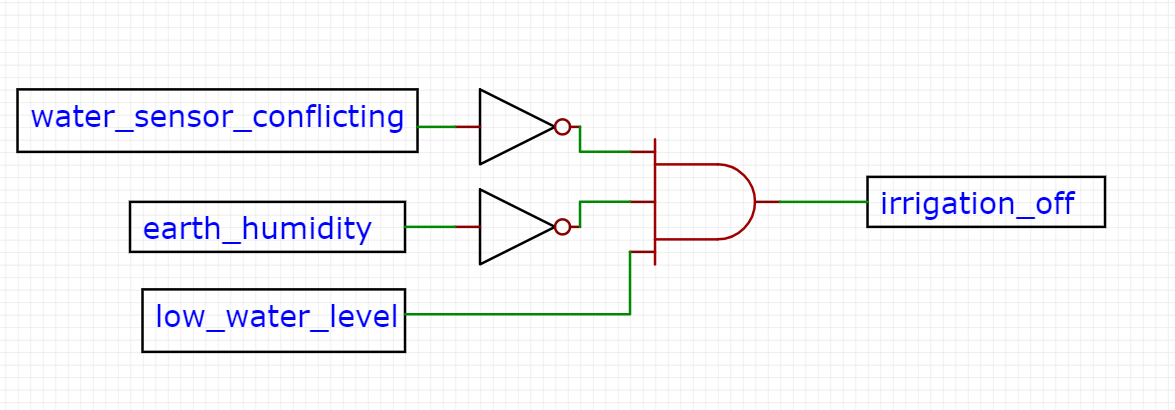
\includegraphics[width=0.75\linewidth]{control-irr.png}
    \caption{Esquema do controlador de irrigação.}
    \label{fig:irr-contrl}
\end{figure}

\subsubsection{Seletor de irrigação}

O módulo \textit{Verilog} \textit{irrigation\_selector} é responsável por determinar qual dos modos de irrigação deverá ser ativo, se aspersor ou gotejador. 
Para isso, deve ser escolhido com base em diferentes condições ambientais e de fornecimento de água. 
Quando sua saída é verdadeira, o modo de aspersão será ativo, do contrário, o modo de gotejamento, essa saída é representada pelo sinal \textit{splinker\_mode\_on}. Existem dois cenários em que o aspersor deve ser ativado:
a) Quando a umidade do ar estiver baixa.
b) Quando a umidade do ar estiver alta, o clima estiver frio e o nível de água estiver acima do nível médio.

Sua tabela verdade está representada pela Tabela \ref{tab:irrigation-selector} e sua simplificação por soma de produtos, pela Equação \eqref{math:irr-selector}, sendo que \textit{A} representa \textit{mid\_water\_level}, \textit{B}, \textit{low\_temperature}, \textit{C}, \textit{air\_humidity} e \textit{Z}, a saída \textit{splinker\_mode\_on}. Sua representação esquemática pode ser vista na Figura \ref{fig:select}.


\begin{table}[h]
\centering
\begin{tabular}{|c|c|c|l|c|}
\hline
\textit{mid\_water\_level} & \multicolumn{1}{l|}{\textit{low\_temperature}} & \textit{air\_humidity} &  & \textit{splinker\_mode\_on} \\ \hline
0 & 0 & 0 &  & 1 \\ \hline
0 & 0 & 1 &  & 0 \\ \hline
0 & 1 & 0 &  & 1 \\ \hline
0 & 1 & 1 &  & 0 \\ \hline
1 & 0 & 0 &  & 1 \\ \hline
1 & 0 & 1 &  & 1 \\ \hline
1 & 1 & 0 &  & 1 \\ \hline
1 & 1 & 1 &  & 0 \\ \hline
\end{tabular}
\caption{Tabela verdade do módulo \textit{irrigation\_selector.v}}
\label{tab:irrigation-selector}
\end{table}



\begin{equation}
\begin{split}
Z &= A'B'C + A'BC' + A'B'C' + AB'C + ABC' \\
Z &= A'C'(B' + B') + A'B'(C' + C) + ABC' \\
Z &= A'C' + AB' + ABC' \\
Z &= A'C' + A(B' + BC') \\
Z &= A'C" + AB' + AC'\\
Z & = C'(A' + A) + AB'\\
Z &= AB' + C'
\label{math:irr-selector}
\end{split}
\end{equation}


\begin{figure}[H]
    \centering
    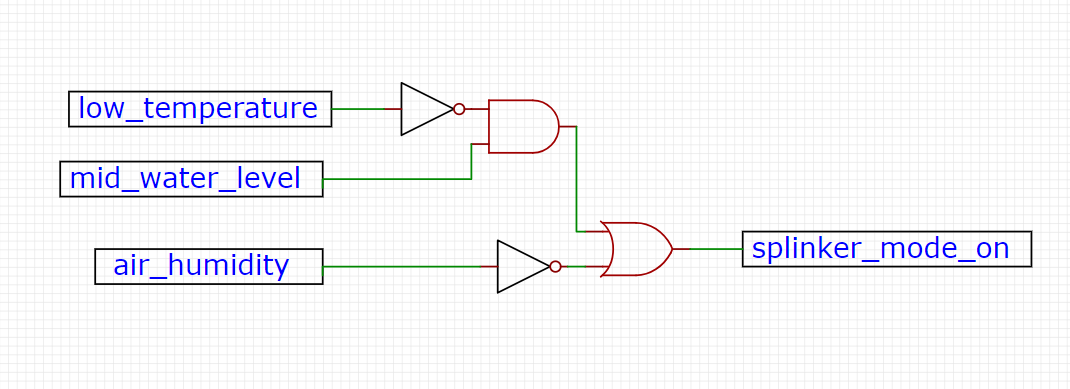
\includegraphics[width=0.75\linewidth]{select.png}
    \caption{Esquema do seletor de irrigação}
    \label{fig:select}
\end{figure}


\subsubsection{Multiplexador 2x1}
O módulo \textit{Verilog} \textit{multiplexer\_2x1.v} é um componente que seleciona entre dois sinais de entrada (\textit{l0} e \textit{l1}) com base no valor de um sinal de seleção \textit{s}, assim como descrito por  \cite{floyd_2007_funes}. O sinal de saída \textit{out} é definido de acordo com o valor de \textit{s}: se \textit{s} for 0, o sinal de saída será igual a \textit{l0}; se \textit{s} for 1, o sinal de saída será igual a \textit{l1}. O processo de seleção é realizado internamente no módulo, garantindo que apenas um dos sinais de entrada seja propagado para o sinal de saída, dependendo do valor de \textit{s}. Seu esquema em diagrama pode ser encontrado na Figura \ref{fig:mux}.

\begin{figure}[H]
    \centering
    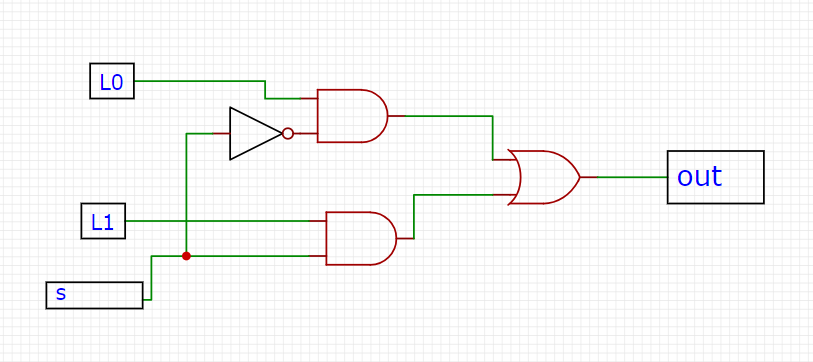
\includegraphics[width=0.75\linewidth]{mux.png}
    \caption{Esquema do Multiplexador 2x1}
    \label{fig:mux}
\end{figure}


\subsubsection{Desabilitador de \textit{display}}

O módulo \textit{disable\_display} é responsável por desabilitar cada grupo do \textit{display} de sete segmentos. Para isso, fora utilizada uma propriedade de simplificação booleana que diz que $A'A = 1$, como pode ser visto na Tabela \ref{tab:disable-display}, portanto o resultado sempre será nível lógico alto, independentemente do valor de $A$. Seu esquema pode ser encontrado na Figura \ref{fig:dis-display}.

\begin{figure}[H]
    \centering
    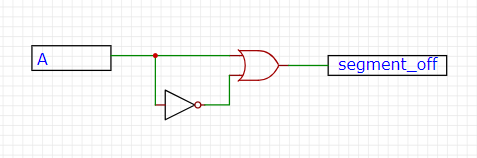
\includegraphics[width=0.75\linewidth]{disabledisplay.png}
    \caption{Esquema do desabilitador de display}
    \label{fig:dis-display}
\end{figure}


\begin{table}[H]
\centering
\begin{tabular}{|c|c|c|}
\hline
\textit{A} &  & segment\_off \\ \hline
0          &  & 1            \\ \hline
1          &  & 1            \\ \hline
\end{tabular}
\caption{Tabela verdade do módulo \textit{disable\_display.v}}
\label{tab:disable-display}
\end{table}

\subsubsection{Seletor do modo de \textit{display}}
O módulo \textit{display\_selector} é um seletor de \textit{display}, implementado como um multiplexador (MUX) em \textit{Verilog}. Ele é responsável por selecionar os dados que serão exibidos em um \textit{display} de sete segmentos com dois bits de entrada. O sinal \textit{selector} determina qual conjunto de dados será enviado para a exibição. Quando \textit{selector} está em estado alto, os bits de entrada \textit{encoded\_irrigation\_Bit1} e \textit{encoded\_irrigation\_Bit0} são selecionados e enviados para os segmentos do display correspondentes. Quando selector está em estado baixo, os bits de entrada \textit{encoded\_water\_Bit1} e \textit{encoded\_water\_Bit0} são selecionados e enviados para o \textit{display}. Esse processo permite alternar entre a exibição dos dados de irrigação e de água no \textit{display}, fornecendo ao usuário as informações necessárias sobre o sistema de irrigação em tempo real.

\subsubsection{Decodificador do \textit{display}}
O módulo \textit{display\_decoder} é responsável por converter os bits de entrada em sinais individuais para cada segmento de um \textit{display} de sete segmentos. Utilizando a lógica booleana, ele interpreta os sinais de entrada \textit{entry\_Bit0} e \textit{entry\_Bit1}, juntamente com o sinal de controle \textit{selector}, para determinar quais segmentos devem ser ativados para representar o valor de entrada. Cada segmento (A, B, C, D, E, F, G) é calculado individualmente com base nos valores dos bits de entrada e no seletor. As operações lógicas de \textit{NOT}, \textit{AND} e \textit{OR} são utilizadas para calcular a ativação de cada segmento de acordo com a combinação de entrada, garantindo que a representação no \textit{display} seja precisa e corresponda ao valor desejado. 

Sua tabela verdade pode ser vista na Tabela \ref{tab:display-decoder}, onde $A$ é o bit menos significativo e $B$ é o mais significativo, ao lado, tem-se as saídas para cada segmento do \textit{display}, enumerados de $a$ a $g$. Já a simplificação de suas expressões podem ser vistas da Equação \eqref{math:display-a} a Equação \eqref{math:display-g}, vale ressaltar que fora utilizado soma de produtos como método principal, exceto pela função $e$, que usou produto de somas. Já a visão esquemática geral pode ser vista na Figura \ref{fig:display}.


\begin{table}[H]
\centering
\begin{tabular}{|c|c|c|c|c|c|c|c|c|c|c|}
\hline
A & B & C &  & a & b & \multicolumn{1}{l|}{c} & \multicolumn{1}{l|}{d} & \multicolumn{1}{l|}{e} & \multicolumn{1}{l|}{f} & \multicolumn{1}{l|}{g} \\ \hline
0 & 0 & 0 &  & 1 & 1 & 1 & 1 & 1 & 1 & 1 \\ \hline
0 & 0 & 1 &  & 1 & 0 & 0 & 1 & 1 & 1 & 1 \\ \hline
0 & 1 & 0 &  & 0 & 0 & 1 & 0 & 0 & 1 & 0 \\ \hline
0 & 1 & 1 &  & 0 & 0 & 0 & 0 & 1 & 1 & 0 \\ \hline
1 & 0 & 0 &  & 1 & 1 & 1 & 1 & 1 & 1 & 1 \\ \hline
1 & 0 & 1 &  & 0 & 0 & 0 & 1 & 0 & 0 & 0 \\ \hline
1 & 1 & 0 &  & 0 & 1 & 0 & 0 & 0 & 0 & 1 \\ \hline
1 & 1 & 1 &  & 1 & 1 & 1 & 1 & 1 & 1 & 1 \\ \hline
\end{tabular}
\caption{Tabela verdade do módulo \textit{display\_decoder.v}}
\label{tab:display-decoder}
\end{table}

\begin{equation}
\begin{split}
a &= A'B'C' + A'B'C + AB'C' + A'B'C' + ABC \\
a &= A'B'(C'+ C) + A(B'C' + BC) + ABC\\
a &= A'B' + AB'C' + ABC\\
a &= B'(A' + AC') + ABC\\
a &= B'(A' + C') + ABC\\
a &= B'A' + BC' + ABC \equiv ABC + B'C' + A'B'
\label{math:display-a}
\end{split}
\end{equation}

\begin{equation}
\begin{split}
b &= A'B'C' + AB'C' + ABC' + ABC  \\
b &= A'B'C' + AB'C' + AB(C' + C)\\
b &= A'B'C' + AB'C' + AB\\
b &= B'C'(A' + A) + AB\\
b &= B'C' + AB
\label{math:display-b}
\end{split}
\end{equation}

\begin{equation}
\begin{split}
c &= A'B'C' + A'B'C' + AB'C' + ABC \\
c &= A'C'(B' + B') + AB'C' + ABC \\
c &= A'C' + AB'C' + ABC \\
c &= C'(A' + AB') + ABC \\
c &= C'(A' + B') + ABC \\
c &= A'C' + B'C' + ABC
\label{math:display-c}
\end{split}
\end{equation}

\begin{equation}
\begin{split}
d &= A'B'C' + A'B'C + AB'C + ABC\\
d &= A'B'(C' + C) + AB'(C' + C) + ABC\\
d &= A'B' + AB' + ABC\\
d &= B'(A + A') + ABC\\
d &= B' + ABC\\
d &= B' + AC
\label{math:display-d}
\end{split}
\end{equation}

\begin{equation}
\begin{split}
e &= A'B'C' + A'B'C + A'BC + AB'C' + ABC\\
e &= A'B'(C' + C) + BC(A' + A) + AB'C'\\
e &= A'B' + BC + AB'C'\\
e &= B'(A' + AC') + BC\\
e &= B'(A' + C') + BC\\
e &= B'A' + B'C' + BC \equiv B'C' + A'C + BC
\label{math:display-e}
\end{split}
\end{equation}

\begin{equation}
\begin{split}
f &= (A' + B + C')(A' + B' + C)\\
f &= (A'A + A'B' + A'C) + (A'B + B'B + BC) + (A'C' + B'C' + CC')\\
f &= (0 + A'B' + A'C) + (A'B + 0 + BC) + (A'C' + B'C' + 0)\\
f &= A'B' + A'C + A'B + BC + A'C' + B'C'\\
f &= A'(B' + B) + A'(C + C') + BC + B'C'\\
f &= A' + A' + BC + B'C'\\
f &= A' + BC + B'C'
\label{math:display-f}
\end{split}
\end{equation}

\begin{equation}
\begin{split}
g &= A'B'C' + A'B'C + AB'C' + ABC' + ABC\\
g &= A'B'(C' + C) + AB'C' + AB(C' + C)\\
g &= A'B' + AB'C' + AB\\
g &= B'(A' + AC') + AB\\
g &= B'(A' + C') + AB\\
g &= A'B' + B'C' + AB
\label{math:display-g}
\end{split}
\end{equation}

\begin{figure}[H]
    \centering
    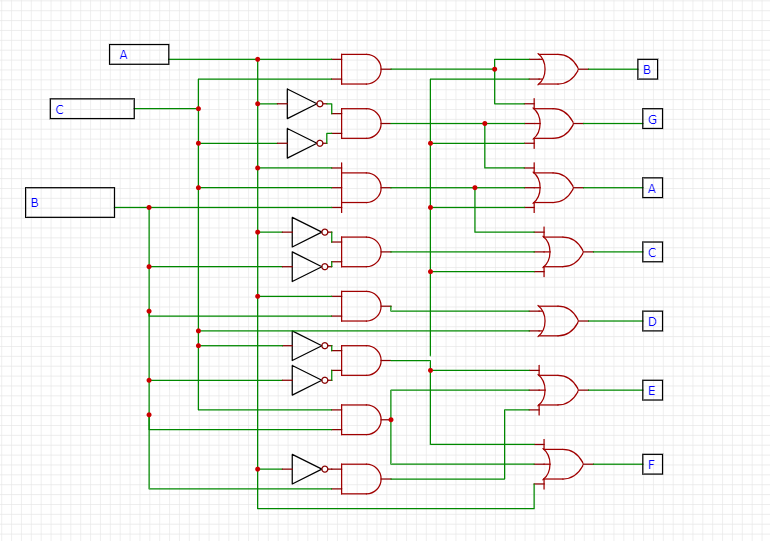
\includegraphics[width=0.75\linewidth]{display.png}
    \caption{Esquema geral do \textit{Display} de 7 Segmentos}
    \label{fig:display}
\end{figure}

\subsection{Pinagem}

Para representar as diferentes situações do circuito, como a abertura das válvulas e os níveis de água na caixa, foram cuidadosamente selecionados os pinos mais apropriados na placa. 
A seguir, descrevemos os pinos selecionados para representar cada uma dessas situações.

Válvula de Entrada: A abertura da válvula de entrada (\textit{Ve}) é representada visualmente pelo \textit{LED0}, localizado no \textit{pino 54} da placa.

Para representar tanto os níveis da caixa d’água quanto os dados dos sensores de umidade do ar, do solo e de temperatura, optou-se por utilizar as \textit{Chaves HH} da placa. 
Desta forma, para garantir o funcionamento completo do circuito, foram atribuídas sete chaves no total.

Os níveis baixo, médio e alto da caixa d’água são representados respectivamente pelas chaves: \textit{CH0}, \textit{CH1} e \textit{CH2}, localizadas nos \textit{pinos 42}, \textit{38} e \textit{30}.
Já os sensores de ambiente, como é o caso dos sensores de umidade do solo, umidade do ar e temperatura foram representados respectivamente pelas chaves \textit{CH3}, \textit{CH4} e \textit{CH5}, localizadas nos \textit{pinos 36}, \textit{34} e \textit{30}.

Além disso, o último pino foi dedicado para alternar o modo de exibição do display de 7 segmentos (\textit{pino 35}), permitindo mostrar o nível da caixa d’água ou o tipo de irrigação (podendo ser aspersão ou gotejamento), conforme selecionado pelo usuário.

As regas de aspersão e Gotejamento foram visualmente representadas em dois locais distintos da placa. 
Inicialmente, optou-se por indicar a ativação dessas regas nos \textit{LEDs LED9} (\textit{pino 76}) para aspersão e \textit{LED8} (\textit{pino 75}) para gotejamento, proporcionando uma visualização direta e acessível. 
Esta escolha permitiu a rápida identificação da ativação das regas, antes mesmo da codificação do \textit{display} de 7 segmentos, facilitando o desenvolvimento do projeto como um todo.

Já o alarme foi integrado ao circuito utilizando o \textit{LED RGB}, configurado para emitir luz vermelha, localizado no \textit{pino 86}.

Além disso, o \textit{display} de segmentos é empregado para representar os tipos de rega, conforme mencionado anteriormente, e o nível da caixa d'água. 
Os segmentos do dígito 3 (último dígito) são utilizados para essa finalidade, com os seguintes pinos associados: \textit{39, 41, 70, 90, 91, 98} e \textit{100}. Não obstante, fora necessário desabilitar partes do \textit{display}, como é o caso do ponto e de dos \textit{displays} à esqueda, para isso, ativando os pinos \textit{66, 68, 88} e \textit{96}.

\subsection{Ferramentas Auxiliares}

No desenvolvimento do projeto, foram implementadas duas ferramentas auxiliares utilizando a linguagem de programação \textit{Python}, versão 3.10. A primeira ferramenta, denominada \textit{clean.py}, tem como função principal a remoção de todos os arquivos temporários gerados durante o uso do software \textit{Quartus II}. Esta operação é essencial para manter a integridade do ambiente de desenvolvimento e evitar a propagação de inconsistências durante o processo de compilação.

A segunda ferramenta, \textit{update\_config.py}, é projetada para automatizar a atualização do arquivo de configuração do \textit{Quartus}. Ela opera lendo um arquivo no formato \textit{TOML} e extrai as variáveis necessárias para configurar adequadamente o ambiente de compilação. As variáveis extraídas incluem a pinagem, o diretório de origem dos módulos e as especificações do dispositivo alvo.

O \textit{script} gerado por esta ferramenta é capaz de configurar a compilação paralela do compilador, definir o dispositivo de destino, adicionar os módulos necessários conforme especificado no diretório de origem, além de configurar a pinagem. Com isso, elimina-se a necessidade de interação manual com o \textit{Pin Planner} do \textit{Quartus}, otimizando o fluxo de trabalho e reduzindo a margem de erro humano.


\section{Resultados}

O circuito sintetizado é relativamente simples, consistindo principalmente de operações lógicas combinacionais e utilizando uma quantidade moderada de recursos do CPLD. Não há armazenamento de estados ou operações sequenciais no circuito, o que pode ser observado pelo fato de não haver nenhum registro (\textit{Register only}) no projeto. 


Assim, ao analisar os resultados da síntese do circuito no \textit{Quartus} é revelado que o projeto utiliza um total de 14 elementos lógicos (LEs) em um \textit{Complex Programmable Logic Device} (CPLD). Todos esses LEs são empregados em operações combinacionais, sem a presença de \textit{flip-flops} ou outros elementos de armazenamento. A distribuição dos LEs por número de entradas nas Tabelas de Verdade mostra uma predominância de operações com múltiplas entradas. Em relação aos pinos de entrada/saída (\textit{I/O pins}), o circuito faz uso de 22 deles. Além disso, o circuito possui um total de 60 \textit{fan-outs}, com uma média de 1.67 \textit{fan-outs} por nó. 

Em relação aos resultados esperados, o projeto alcançou sucesso em todas as métricas estabelecidas, satisfazendo integralmente os requisitos técnicos para o circuito. Este êxito não apenas demonstra a eficácia do sistema automatizado de irrigação desenvolvido, mas também reforça a importância da adequada preparação e capacitação técnica na execução de projetos complexos em Sistemas Digitais.
% ---
% Finaliza a parte no bookmark do PDF, para que se inicie o bookmark na raiz
% ---
\bookmarksetup{startatroot}% 
% ---

% ---
% Conclusão
% ---
\section*{Considerações finais}
\addcontentsline{toc}{section}{Considerações finais}

No desenvolvimento do projeto, os desafios mais significativos estiveram relacionados ao processo de aprendizagem das tecnologias e metodologias aplicadas. Embora estes desafios sejam intrínsecos ao processo de pesquisa e desenvolvimento, eles não são o foco principal deste relatório. 

A concepção do circuito abordou diversos aspectos cruciais para seu funcionamento eficiente. Cada módulo, desde o alarme até o controlador de irrigação, foi cuidadosamente projetado para atender aos requisitos específicos do sistema. A análise dos resultados da síntese do circuito no \textit{Quartus} demonstrou que o projeto alcançou sucesso em todas as métricas estabelecidas, utilizando um número moderado de recursos do CPLD. Essa eficiência confirma a importância da preparação técnica adequada na execução de projetos complexos em Sistemas Digitais. A integração harmoniosa dos diferentes módulos resultou em um sistema robusto e confiável, capaz de atender às necessidades de irrigação residencial de forma sustentável e eficaz.

% \lipsum[1]

% % \begin{citacao}
% % \lipsum[2]
% % \end{citacao}

% \lipsum[3]

% ----------------------------------------------------------
% ELEMENTOS PÓS-TEXTUAIS
% ----------------------------------------------------------
\postextual

% ---
% Título e resumo em língua estrangeira
% ---

% \twocolumn[    		% INICIO DE ARTIGO EM DUAS COLUNAS

% titulo em inglês
\titulo{Problema 1: Rega Automatizada!}
\emptythanks
\maketitle

% resumo em português
\renewcommand{\resumoname}{Abstract}
\begin{resumoumacoluna}
 \begin{otherlanguage*}{english}
   This report aims to present the methodology and development of an automated irrigation system. The system was designed to optimize water usage in crops, aiming to enhance economic efficiency compared to traditional irrigation methods. Using the Verilog structural programming language and \textit{Quartus software}, the system was implemented on a \textit{CPLD MAX II} board. The achieved results confirmed the project's success, demonstrating the technical feasibility and operational effectiveness of the proposed system. Additionally, the project contributed to the consolidation of theoretical knowledge related to Digital Systems, aligning with existing literature and suggesting paths for future research and practical applications in the field of agricultural automation.

   \vspace{\onelineskip}
 
   \noindent
   \textbf{Key-words}: automated irrigation. digital circuits. Verilog. Quartus. CPLD MAX II. water efficiency. digital systems. agricultural technology.






 \end{otherlanguage*}  
\end{resumoumacoluna}

% ]  				% FIM DE ARTIGO EM DUAS COLUNAS
% ---

% ----------------------------------------------------------
% Referências bibliográficas
% ----------------------------------------------------------
\bibliography{abntex2-modelo-references}

\end{document}
